\documentclass[border=1pt]{standalone}
%\usetikzlibrary{...}% tikz package already loaded by 'tikz' option
\usepackage{tikz}
\usetikzlibrary{matrix, fit}
\usetikzlibrary{backgrounds}
\begin{document}
\thispagestyle{empty}
$
\hspace{-10pt}
\vcenter{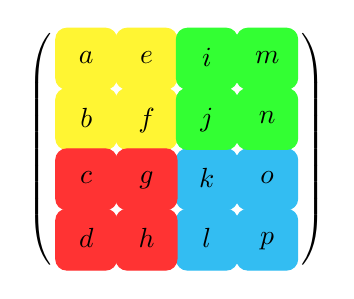
\begin{tikzpicture}
\matrix [matrix of math nodes,
         nodes={rectangle, 
                minimum size=2.2em, text depth=0.25ex,
                inner sep=0pt, outer sep=0pt,
                anchor=center},
         column sep=-0.5\pgflinewidth,
         row sep=-0.5\pgflinewidth,
         inner sep=0pt,
         left delimiter=(, right delimiter=),
         ] (m)
{
a &  e &  i &  m    \\
b &  f & j  &  n   \\
 c &  g &  k&  o  \\
d &  h &  l &  p  \\
};
\begin{scope}[on background layer]
    \filldraw[cyan!80, rounded corners] (m-3-4.north west) -- 
        (m-3-4.north east) -- (m-3-4.south east)-- (m-3-4.south west)-- 
        cycle;
    \filldraw[cyan!80, rounded corners] (m-3-3.north west) -- 
        (m-3-3.north east) -- (m-3-3.south east)-- (m-3-3.south west)-- 
        cycle;
    \filldraw[cyan!80, rounded corners] (m-4-4.north west) -- 
        (m-4-4.north east) -- (m-4-4.south east)-- (m-4-4.south west)-- 
        cycle;
    \filldraw[cyan!80, rounded corners] (m-4-3.north west) -- 
        (m-4-3.north east) -- (m-4-3.south east)-- (m-4-3.south west)-- 
        cycle;
        %%%
    \filldraw[yellow!80, rounded corners] (m-1-2.north west) -- 
        (m-1-2.north east) -- (m-1-2.south east)-- (m-1-2.south west)-- 
        cycle;
    \filldraw[yellow!80, rounded corners] (m-1-1.north west) -- 
        (m-1-1.north east) -- (m-1-1.south east)-- (m-1-1.south west)-- 
        cycle;
    \filldraw[yellow!80, rounded corners] (m-2-2.north west) -- 
        (m-2-2.north east) -- (m-2-2.south east)-- (m-2-2.south west)-- 
        cycle;
    \filldraw[yellow!80, rounded corners] (m-2-1.north west) -- 
        (m-2-1.north east) -- (m-2-1.south east)-- (m-2-1.south west)-- 
        cycle;
        %%%
    \filldraw[green!80, rounded corners] (m-1-4.north west) -- 
        (m-1-4.north east) -- (m-1-4.south east)-- (m-1-4.south west)-- 
        cycle;
    \filldraw[green!80, rounded corners] (m-1-3.north west) -- 
        (m-1-3.north east) -- (m-1-3.south east)-- (m-1-3.south west)-- 
        cycle;
    \filldraw[green!80, rounded corners] (m-2-4.north west) -- 
        (m-2-4.north east) -- (m-2-4.south east)-- (m-2-4.south west)-- 
        cycle;
    \filldraw[green!80, rounded corners] (m-2-3.north west) -- 
        (m-2-3.north east) -- (m-2-3.south east)-- (m-2-3.south west)-- 
        cycle;
        %%%
    \filldraw[red!80, rounded corners] (m-3-2.north west) -- 
        (m-3-2.north east) -- (m-3-2.south east)-- (m-3-2.south west)-- 
        cycle;
    \filldraw[red!80, rounded corners] (m-3-1.north west) -- 
        (m-3-1.north east) -- (m-3-1.south east)-- (m-3-1.south west)-- 
        cycle;
    \filldraw[red!80, rounded corners] (m-4-2.north west) -- 
        (m-4-2.north east) -- (m-4-2.south east)-- (m-4-2.south west)-- 
        cycle;
    \filldraw[red!80, rounded corners] (m-4-1.north west) -- 
        (m-4-1.north east) -- (m-4-1.south east)-- (m-4-1.south west)-- 
        cycle;
\end{scope} 
\end{tikzpicture}}\hspace{-170pt}
$
\end{document}